\pagestyle{fancy}
\pagenumbering{arabic}

\section{Topic and Introduction}
\label{sec:Topic_and_Introduction}
In manufacturing companies, the proper assembly line plays a crucial role in ensuring efficient production processes and meeting customer demand. Nevertheless, with wrong assembly line configurations, companies may face challenges such as high production costs, low productivity, and delays. In the shopfloor of a manufacturing facility, assembly line balancing is therefore a crucial process that aims to optimise the allocation of tasks among workers and machines (Friedli et al., 2010). This process ensures that the assembly line operates efficiently and effectively, maximising productivity while minimising bottlenecks and idle time. There are several models in order to optimise and balance assembly lines, including the mixed model line balancing approach (Yusuf et al., 2020). This approach aims to balance the workload and maximise efficiency in assembly lines where multiple product models are being produced. The mixed model line balancing approach takes into consideration various factors such as workstation requirements, cycle times, and demand variability to determine the optimal allocation of tasks across workstations in order to prevent idle time. To address this challenge, we developed a software tool using Python programming language to faciliate the process of assembly line balancing for mixed model production. 

\section{Project Management}
In order to obtain a proper structure to fulfil the project requirements, we developed the known project management tools studied in the previous semesters. Those tools helped us to dissect different tasks and distribute them.

\subsection{Magic Triangle}
After gaining some theoretical knowledge of the course in the first weeks, we started developing our project on the 27th of October, 2023. In the beginning, we had to choose a project by the given list or come up with our own idea. We decided to take that into account and develop a tool which should help fellow students to gain more knowledge in the topic around the assembly line production. For that, we had resources of 90 workload hours per person which should help us achieve the desired goals. Regarding the sources we were able to use, there were no boundaries which allows us to gain the theoretical knowledge of assembly line balancing through literature of scientific papers as well as materials from previous semesters where we talked about the assembly line production in detail. In the development of the Python tool for the practical part, we will primarily conduct internet research, as it proved to be a more time-efficient approach for addressing our specific issue. Additionally, we set biweekly meetings with our stakeholder which should help us developing the tool by talking about what features should be applied and how to make it as user-friendly as possible for students. Within the group, we are gonna implement those by meeting each other once a week and also think about how else to improve the tool. 
\begin{figure}[H]
\centering
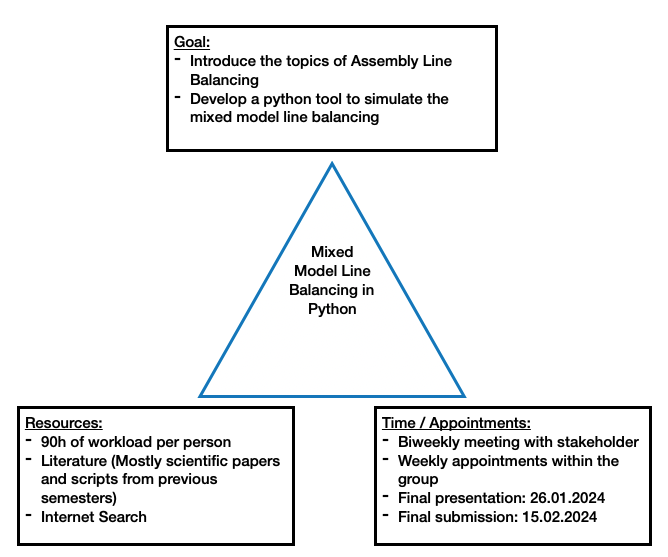
\includegraphics[width=10cm]{Abbildungen/Magic_Triangle_start.png}	
\caption{Magic Triangle (27.10.2023)}
\label{fig:Magic_Triangle_start}
\end{figure}
\noindent
After finishing and refining our tool, we drew the magic triangle once again in comparison to the initiative one. As to be seen the triangle with the red border filled with blue, demonstrates our changes. For that, the most change that took place belongs to the category of resources. Especially by taking a look at our workload hours we invested more time than was initially planned. By an extension 20h per person, it allowed us to develop the tool as desired. This was necessary for the reason that we never learned how to build a tool with a graphical user interface. We allocated the additional time for gaining the Know-How which also lead to the change of our weekly appointments to two-day-meetings. The goal as well as the dates of submission did not vary. For that reason, the modified triangle mostly shifted to the left since it had the biggest impact of our project process.
\begin{figure}[H]
\centering
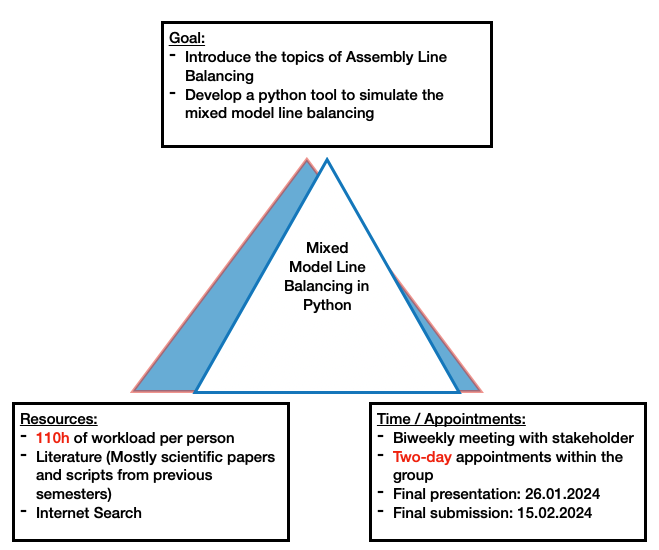
\includegraphics[width=10cm]{Abbildungen/Magic_Triangle_end.png}
\caption{Magic Triangle (24.01.2024)}
\label{fig:Magic_Triangle_end}
\end{figure}
\subsection{Gantt-Chart}
Another project management tool we applied was the Gantt-Chart. Here, the stations of our project process can be seen in much more detail then in the magic triangle. The length of the bars in the diagram are linked to the duration of how long each station took. As to be seen, the creation and definition of our objectives had a big impact on our project. The reason for that was the lack of clarity within the group and the vague definition of what we want to achieve with the tool. By talking with our stakeholder Prof. Dr.-Ing. Nicole Stricker at the first meeting, we clarified the objectives and refined what we want to implement within the tool. Another big factor regarding the length is the implementation of our already developed code to Visual Studio Code (VSC). This had to be done in order to achieve the graphical user interface (GUI) so students do not necessarily see our code and can execute our tool by simply executing an application. Not only building the first frame and brainstorming how the GUI should look like took us some time but also doing researches on how to actually perform a GUI in Python since we haven't done that so far. One advantage was that we already studied the basics of Python in the previous semesters through different projects and also this semester helped us gaining more knowledge of how to set up dataframes. 
\begin{figure}[H]
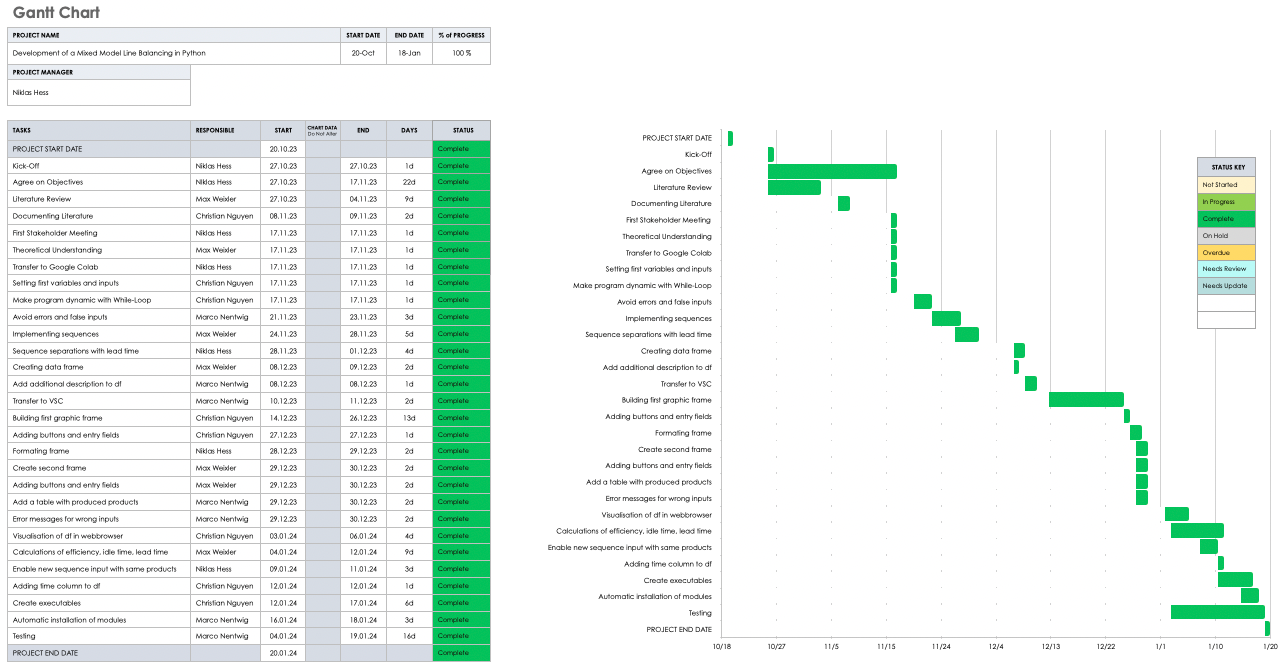
\includegraphics[width=\linewidth]{Abbildungen/Gantt_Chart.png}	
\caption{Gantt-Chart}
\label{fig:Gantt_Chart}
\end{figure}
\section{Results}

